\section{Introduction}

The \textit{proceedings} are the records of a conference.\footnote{This
  is a footnote}  ACM seeks
to give these conference by-products a uniform, high-quality
appearance.  To do this, ACM has some rigid requirements for the
format of the proceedings documents: there is a specified format
(balanced double columns), a specified set of fonts (Arial or
Helvetica and Times Roman) in certain specified sizes, a specified
live area, centered on the page, specified size of margins, specified
column width and gutter size.

\section{The Body of The Paper}


\begin{table*}
  \caption{Some Typical Commands}
  \label{tab:commands}
  \begin{tabular}{ccl}
    \toprule
    Command &A Number & Comments\\
    \midrule
    \texttt{{\char'134}author} & 100& Author \\
    \texttt{{\char'134}table}& 300 & For tables\\
    \texttt{{\char'134}table*}& 400& For wider tables\\
    \bottomrule
  \end{tabular}
\end{table*}
% end the environment with {table*}, NOTE not {table}!


%\begin{figure}
%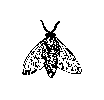
\includegraphics[height=1in, width=1in]{fly}
%\caption{A sample black and white graphic
%that has been resized with the \texttt{includegraphics} command.}
%\end{figure}


As was the case with tables, you may want a figure that spans two
columns.  To do this, and still to ensure proper ``floating''
placement of tables, use the environment \textbf{figure*} to enclose
the figure and its caption.  And don't forget to end the environment
with \textbf{figure*}, not \textbf{figure}!

%\begin{figure*}
%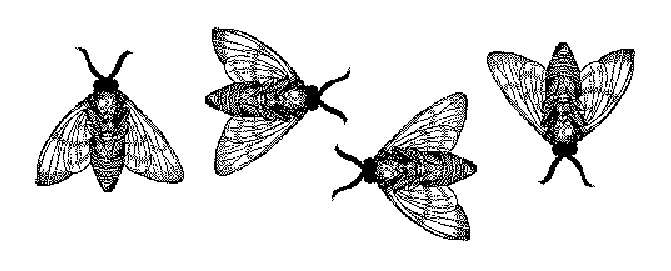
\includegraphics{flies}
%\caption{A sample black and white graphic
%that needs to span two columns of text.}
%\end{figure*}


%\begin{figure}
%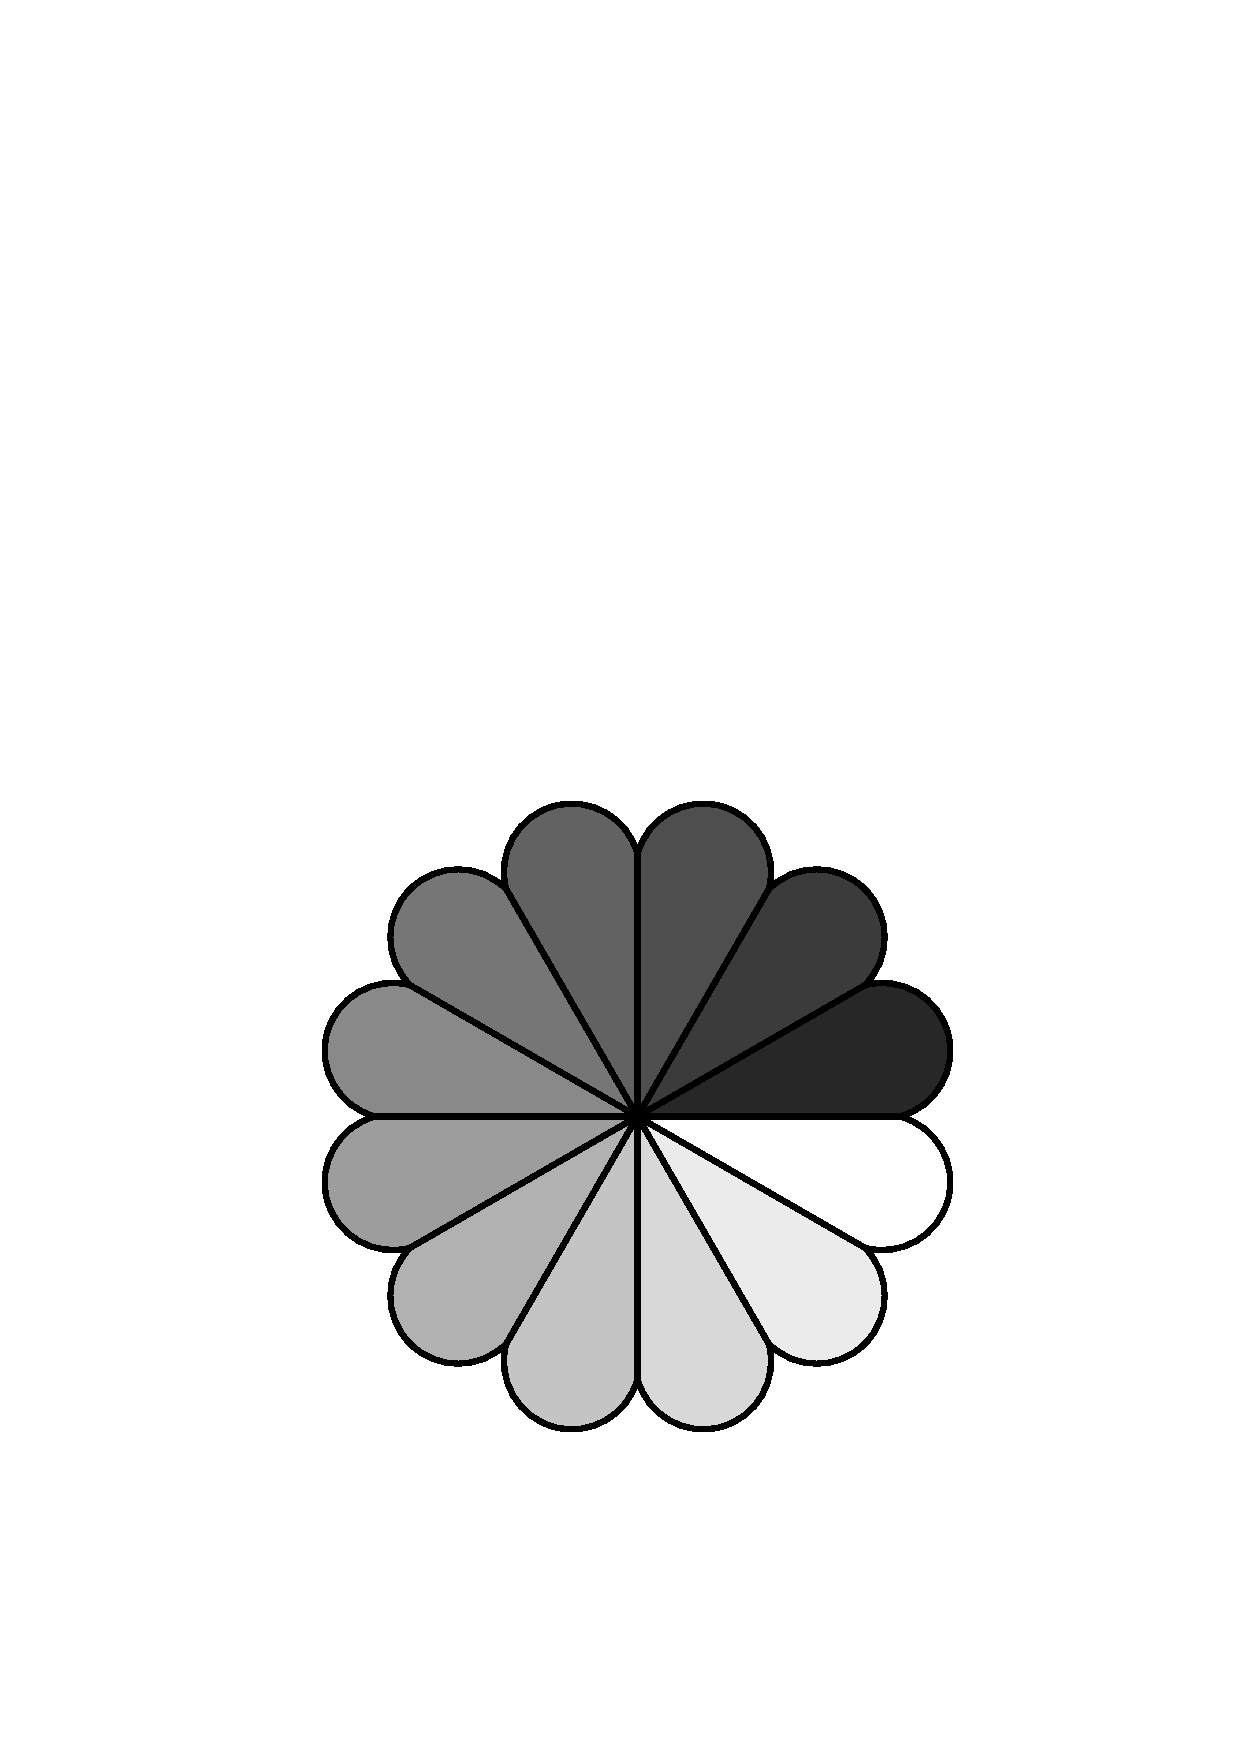
\includegraphics[height=1in, width=1in]{rosette}
%\caption{A sample black and white graphic that has
%been resized with the \texttt{includegraphics} command.}
%\end{figure}

\subsection{Experiment}
\label{sec:exp_results}
Having a multi-population based algorithm can decrease the execution time
because of the parallel execution of the evolution. But, having heterogeneous 
populations might enhance evolutionary search and needless
evaluations than homogeneous systems; heterogeneous settings, if
done right, increases the diversity of the whole population
\cite{araujo2008multikulti}.

But this is a rule of thumb, and it will depend on the degree of heterogeneity,
as well as on the algorithm itself. Some level of heterogeneity can be
implemented by just changing the configuration parameters of each population,
but in this case, we are interested in a heterogeneous search strategy. 
Therefore, in this experiment we compare a multi-population with only GA and PSO populations,
versus an ensemble of GA and PSO algorithms. We tested on the first five functions of the
BBOB testbed. We used ten populations and eight workers for the experiment and the
same parameters as before.  


\begin{figure*}[h!tb]
    \begin{tabular}
        {c@{\hspace*{-0.00001\textwidth}}
         c@{\hspace*{-0.00001\textwidth}}
         c@{\hspace*{-0.00001\textwidth}}
        }
    GA  &  PSO & GA \& PSO\\   
    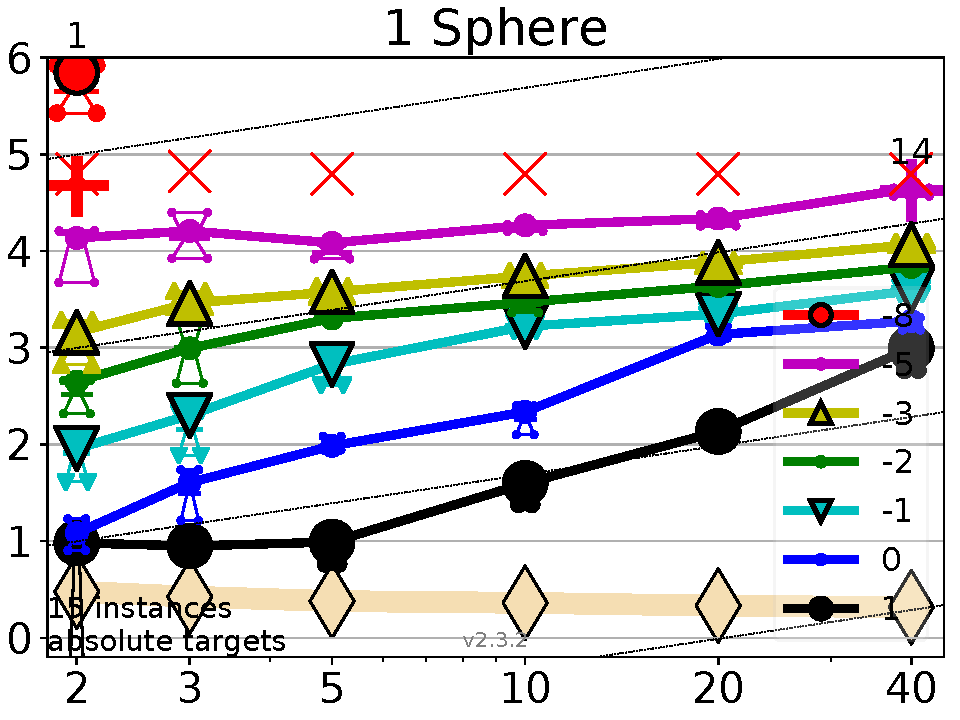
\includegraphics[width=0.28\textwidth]{GAOnly_f001}&
    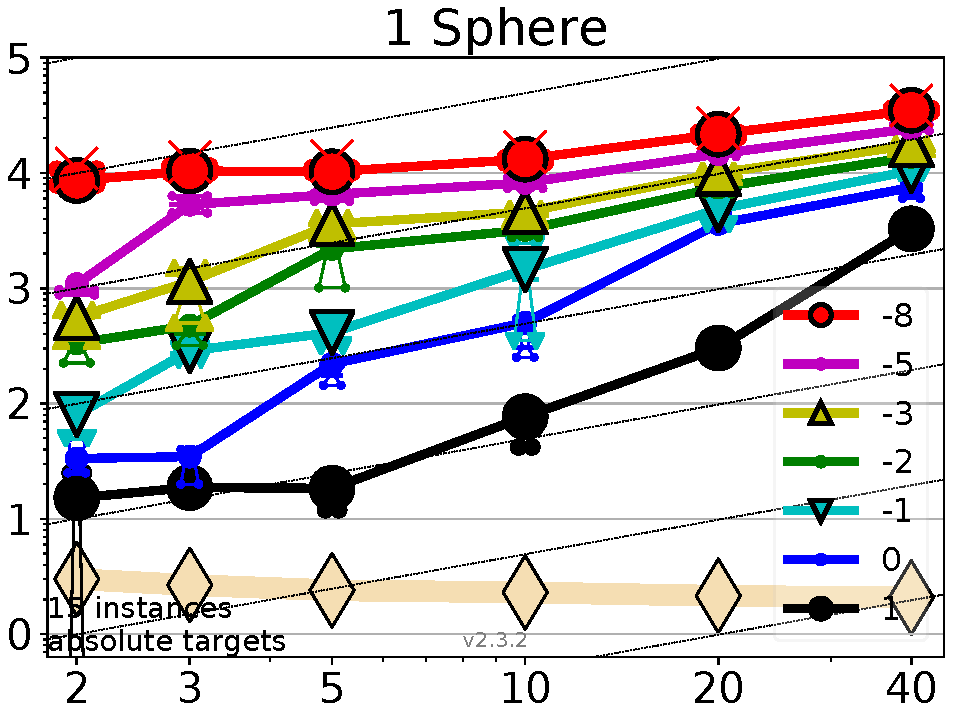
\includegraphics[width=0.28\textwidth]{PSOOnly_f001}&
    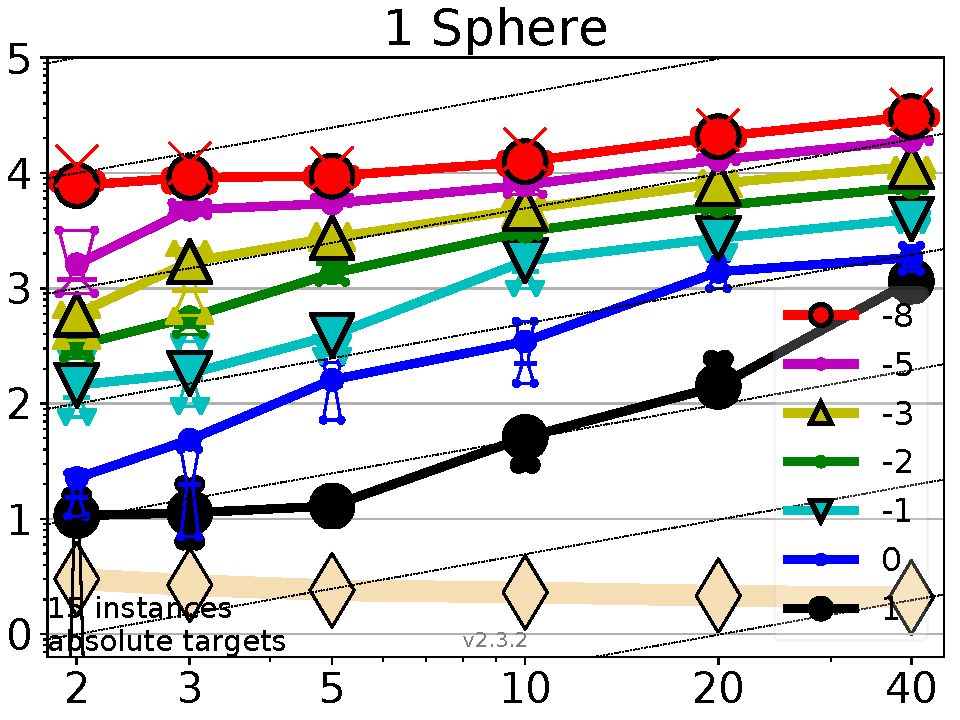
\includegraphics[width=0.28\textwidth]{GAPSO_f001}\\

    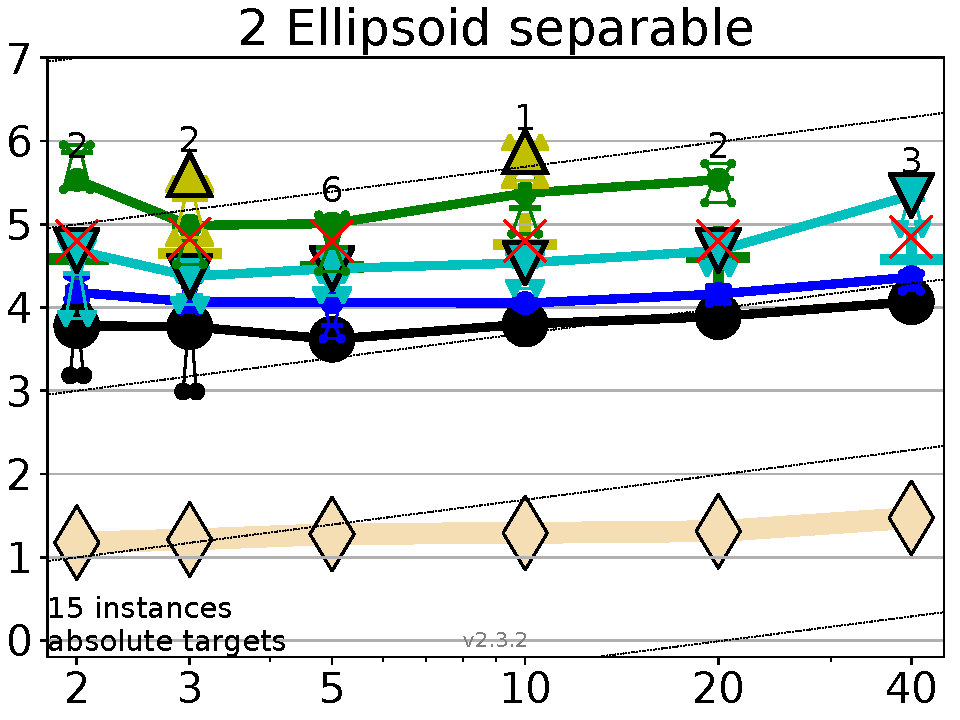
\includegraphics[width=0.28\textwidth]{GAOnly_f002}&
    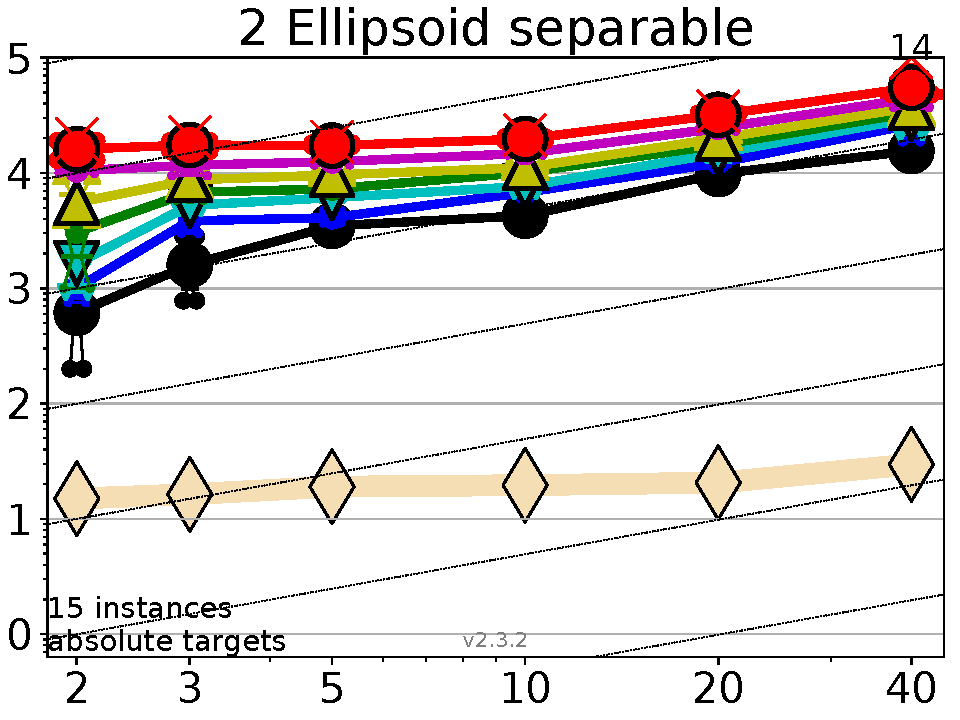
\includegraphics[width=0.28\textwidth]{PSOOnly_f002}&
    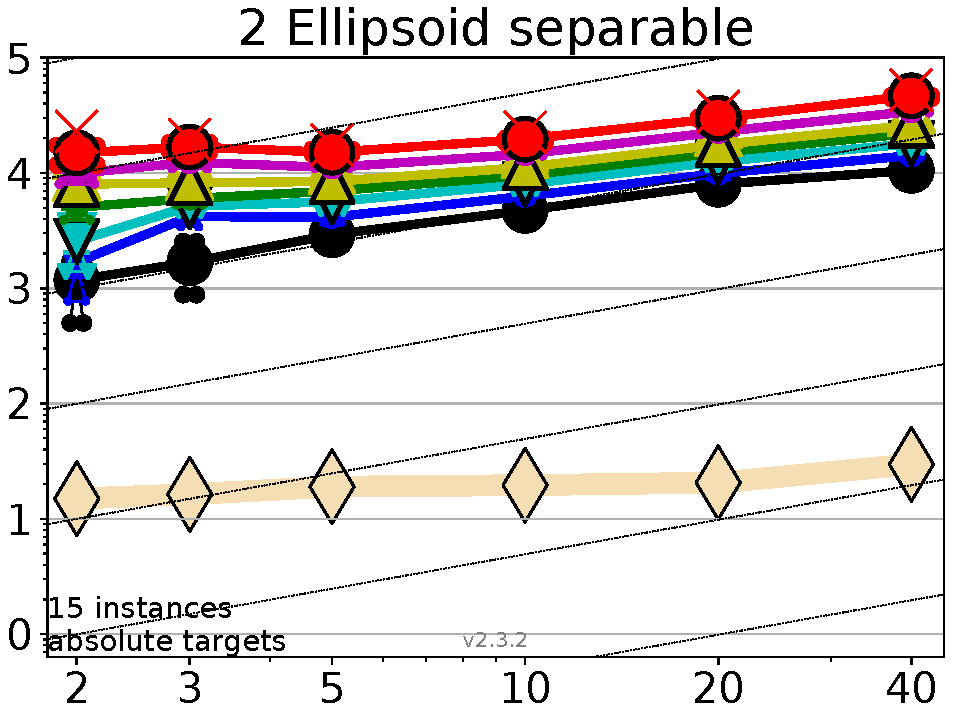
\includegraphics[width=0.28\textwidth]{GAPSO_f002}\\

    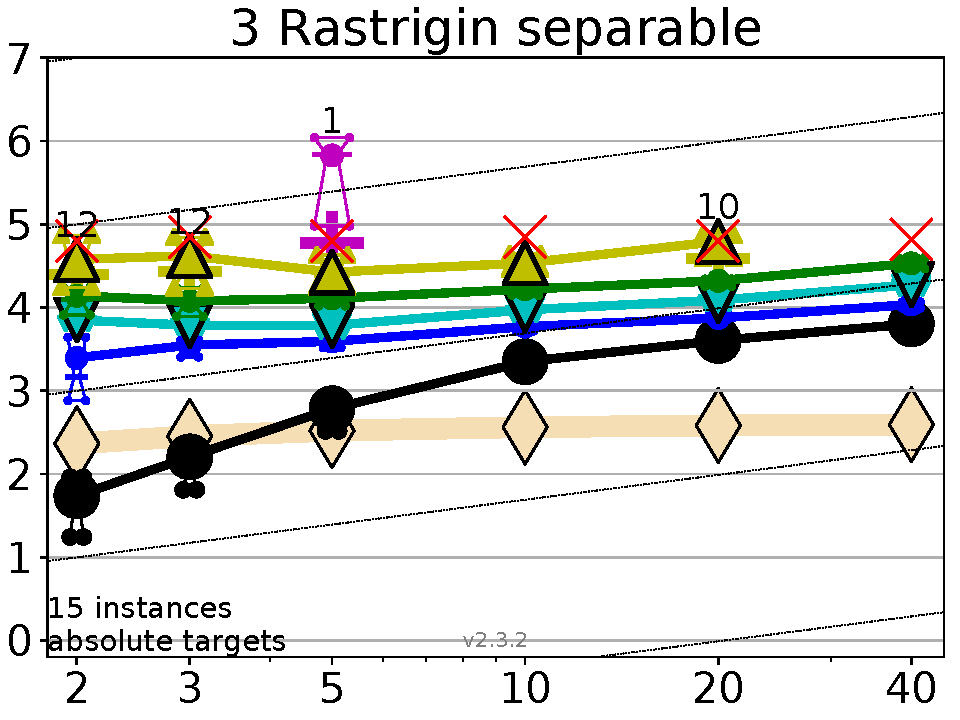
\includegraphics[width=0.28\textwidth]{GAOnly_f003}&
    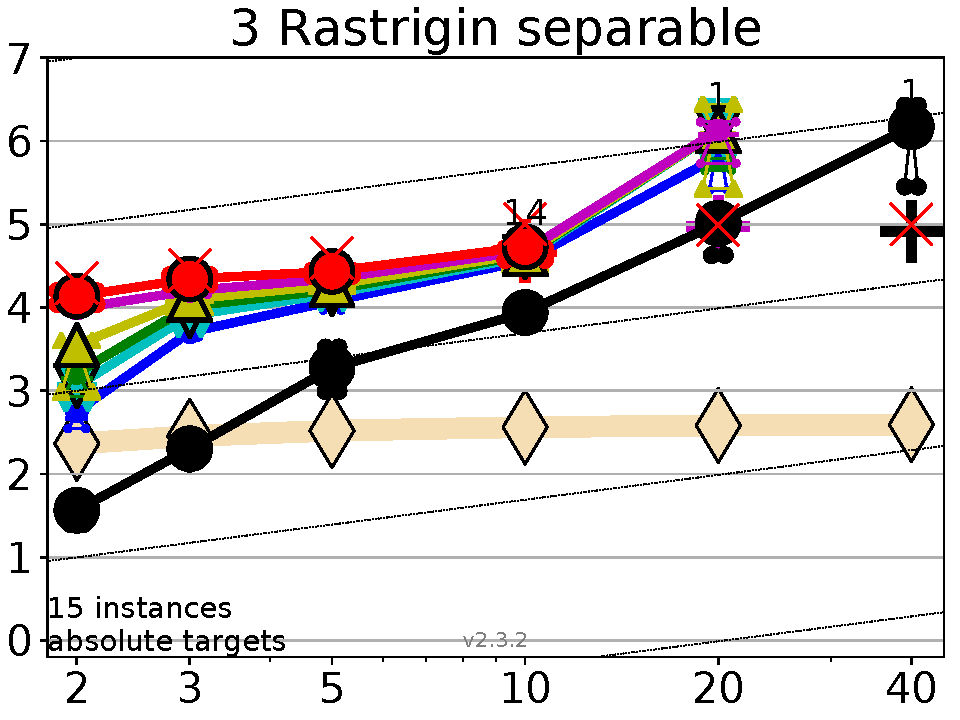
\includegraphics[width=0.28\textwidth]{PSOOnly_f003}&
    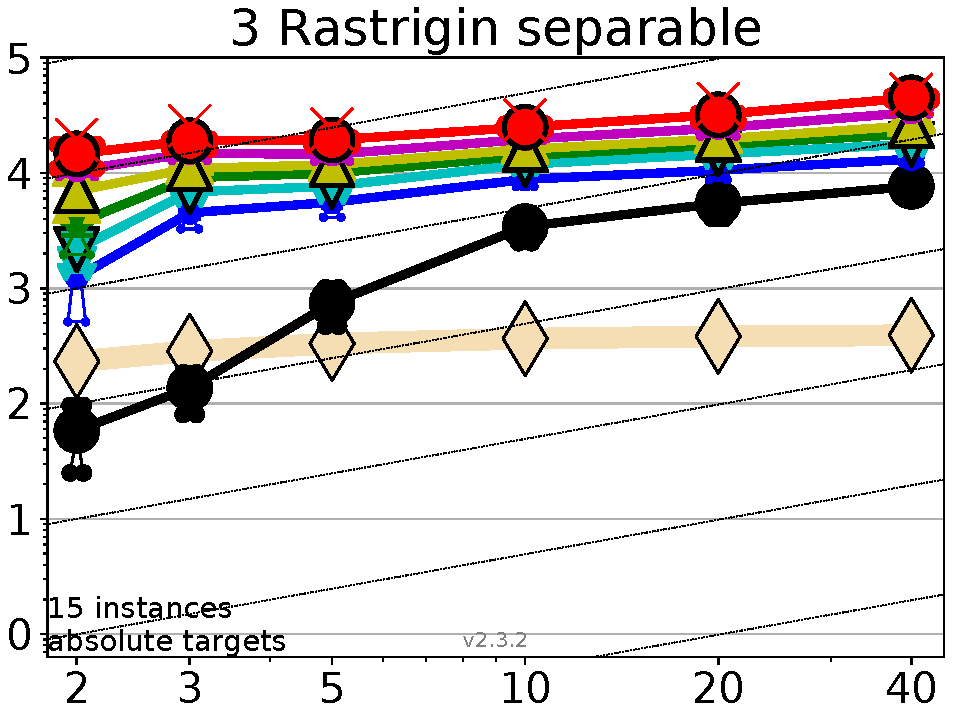
\includegraphics[width=0.28\textwidth]{GAPSO_f003}\\

    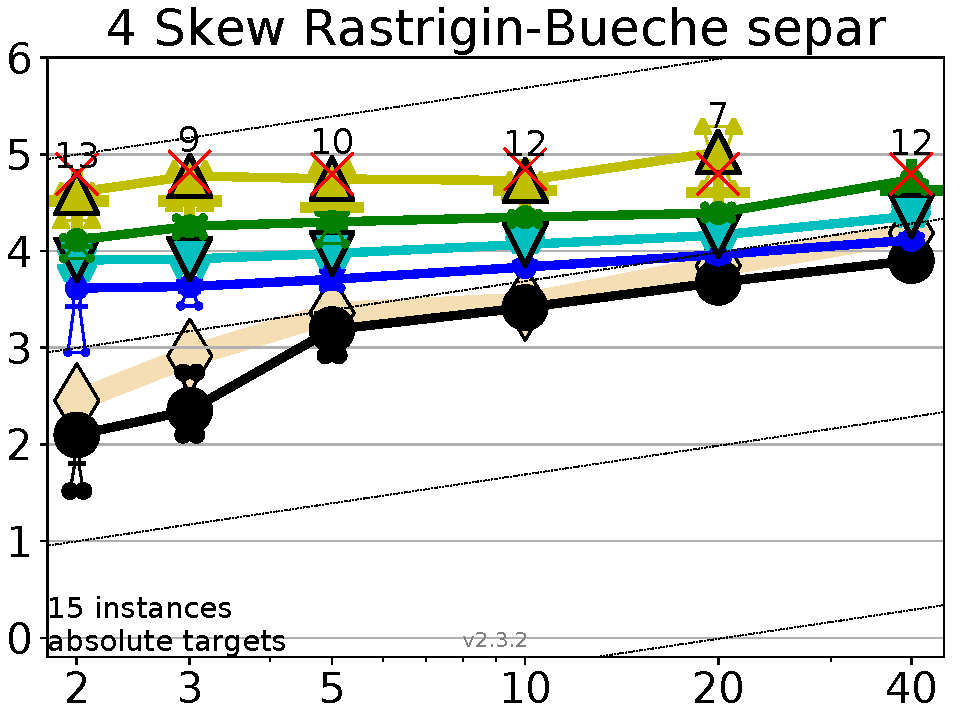
\includegraphics[width=0.28\textwidth]{GAOnly_f004}&
    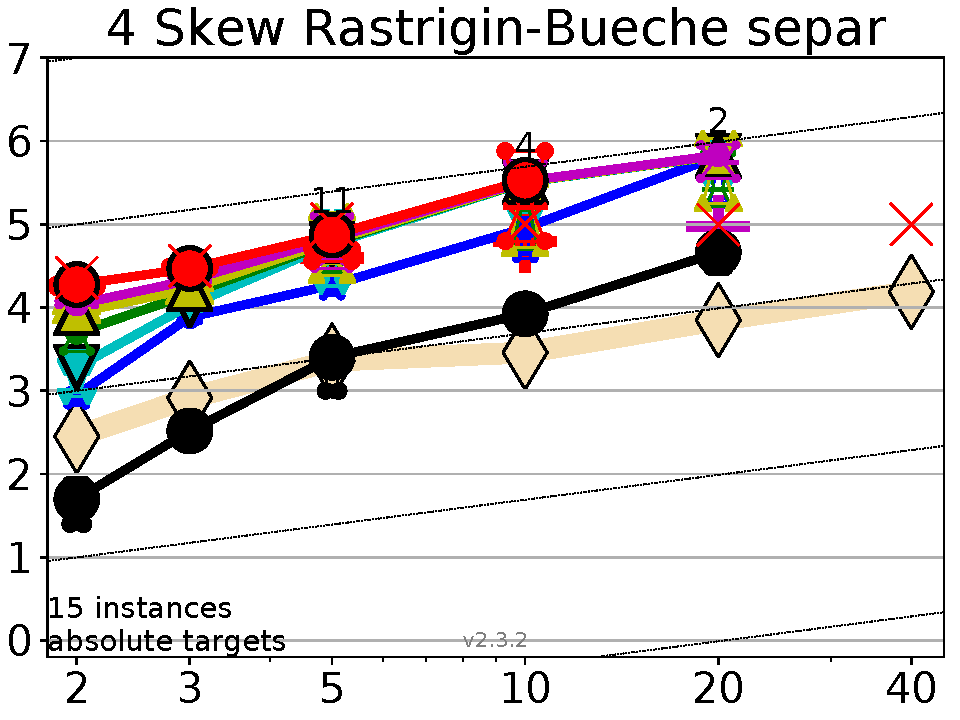
\includegraphics[width=0.28\textwidth]{PSOOnly_f004}&
    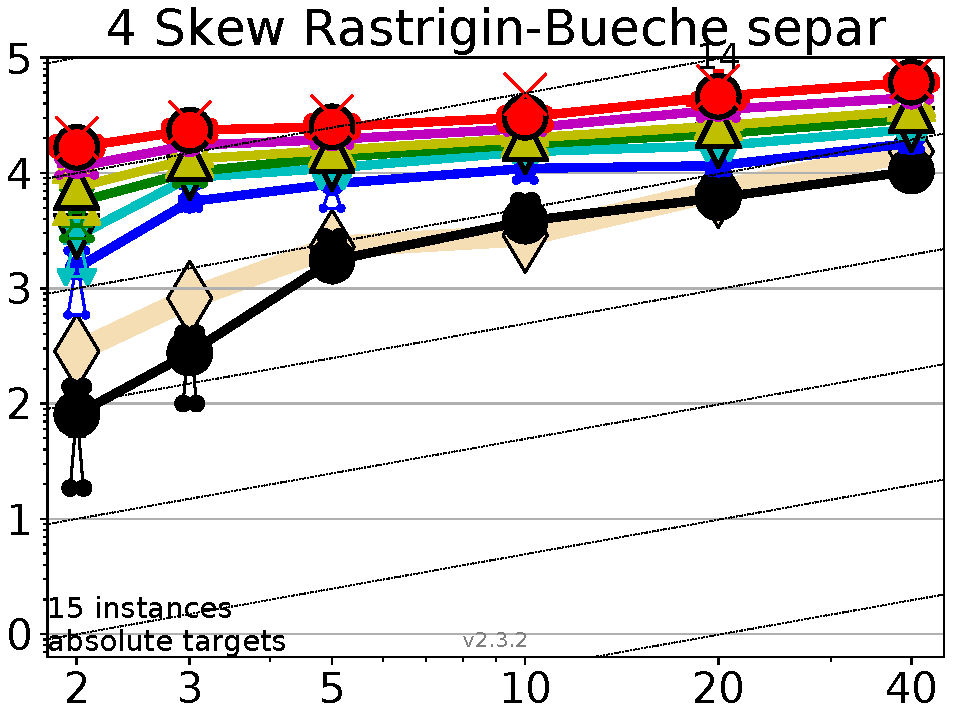
\includegraphics[width=0.28\textwidth]{GAPSO_f004}\\

    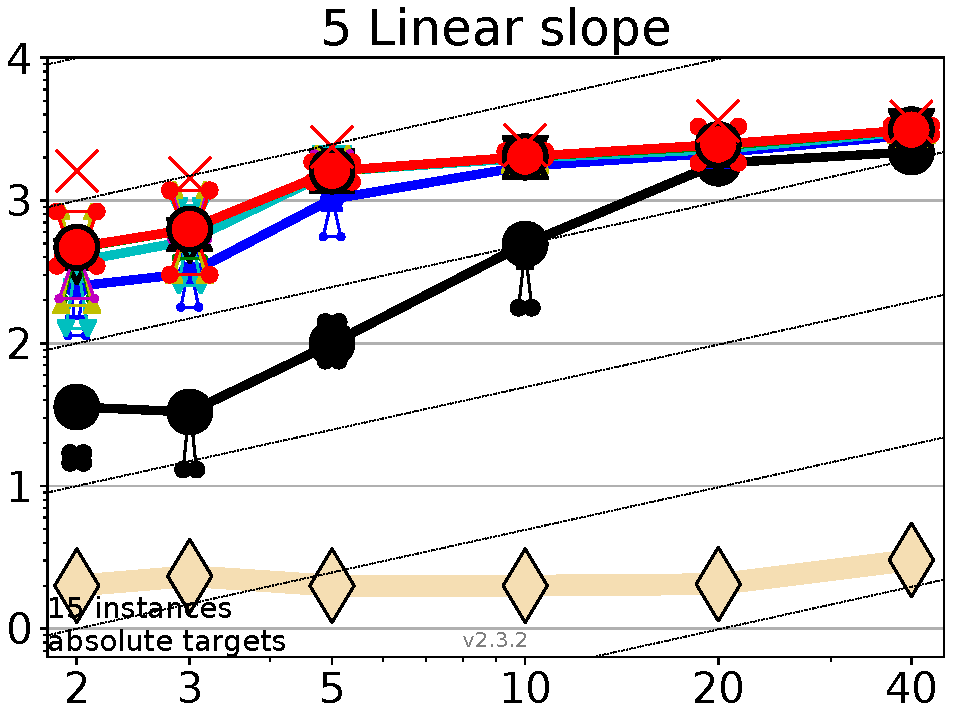
\includegraphics[width=0.28\textwidth]{GAOnly_f005}&
    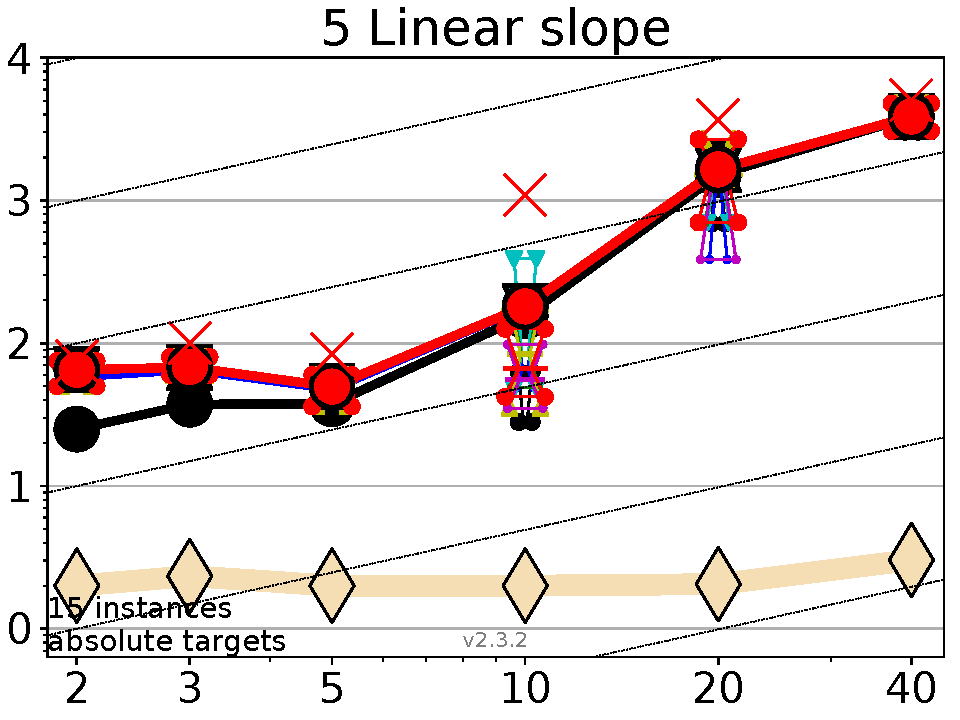
\includegraphics[width=0.28\textwidth]{PSOOnly_f005}&
    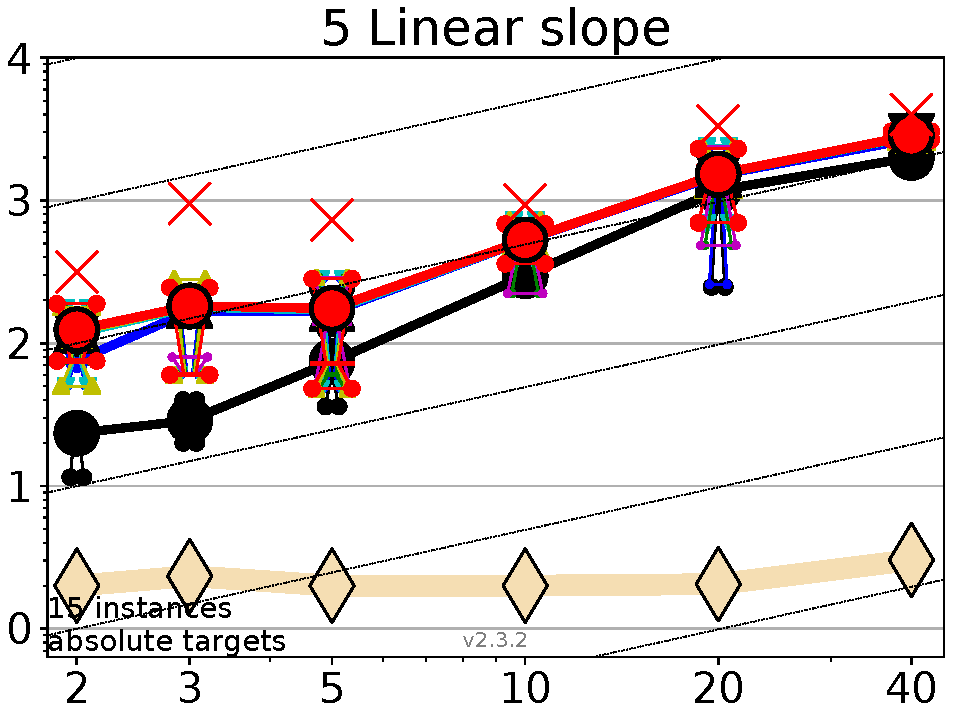
\includegraphics[width=0.28\textwidth]{GAPSO_f005}\\
    \end{tabular}
    \vspace{-3ex}
     \caption{
 Scaling of runtime with dimension to reach certain target values $\Delta f$. Lines:
 average runtime (aRT); Cross ($+$): median runtime of successful runs to reach
 the most difficult target that was reached at least once (but not always);
 Cross (\textcolor{red}{$\times$}): maximum number of f-evaluations in any trial. Notched boxes:
 interquartile range with median of simulated runs; All values are divided by
 dimension and plotted as $log_{10}$ values versus dimension. 
 %Shown is the aRT for
 %fixed values of $\Delta f = 10k$ with $k$ given in the legend. 
 Numbers above aRT-symbols
 (if appearing) indicate the number of trials reaching the respective target.
 %The light thick line with diamonds indicates the best algorithm from BBOB 2009
 %for the most difficult target. Horizontal lines mean linear scaling, slanted
 %grid lines depict quadratic scaling.
 }
    \end{figure*}


    \begin{figure}[h!tb]
        \begin{tabular}
            {c@{\hspace*{-0.00001\textwidth}}
            % c@{\hspace*{-0.00001\textwidth}}
            }
           
        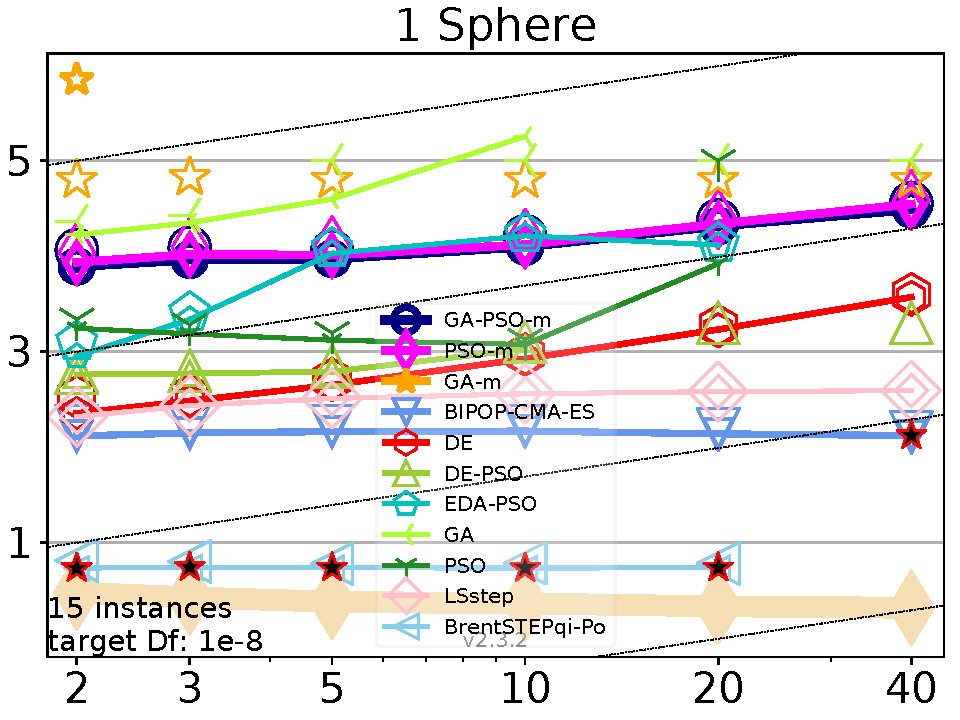
\includegraphics[width=0.28\textwidth]{ppfigs_f001}\\
        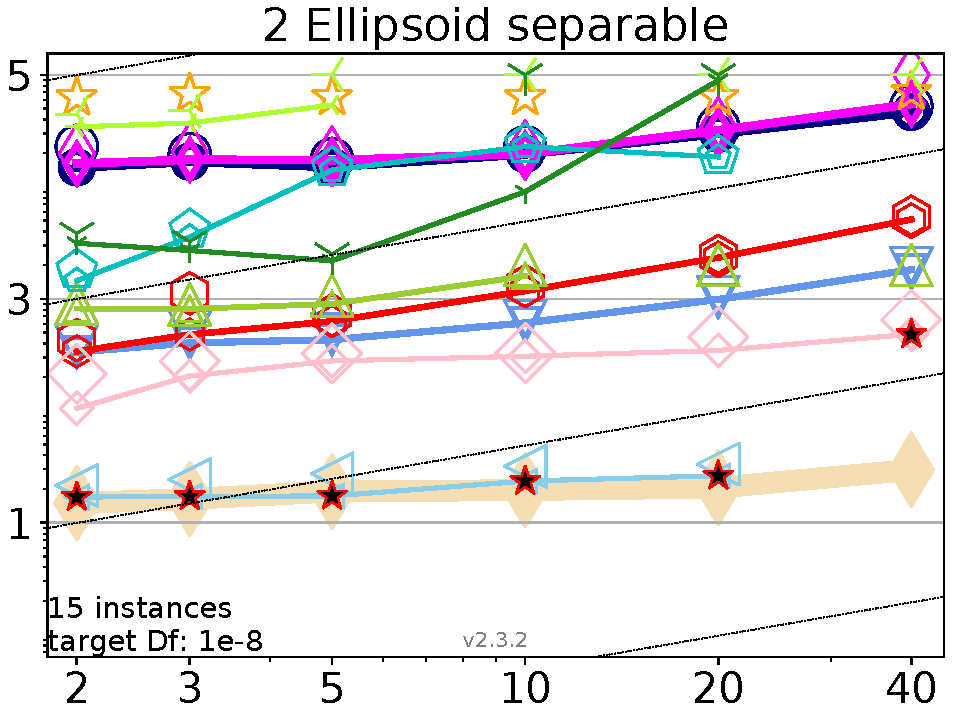
\includegraphics[width=0.28\textwidth]{ppfigs_f002}\\

        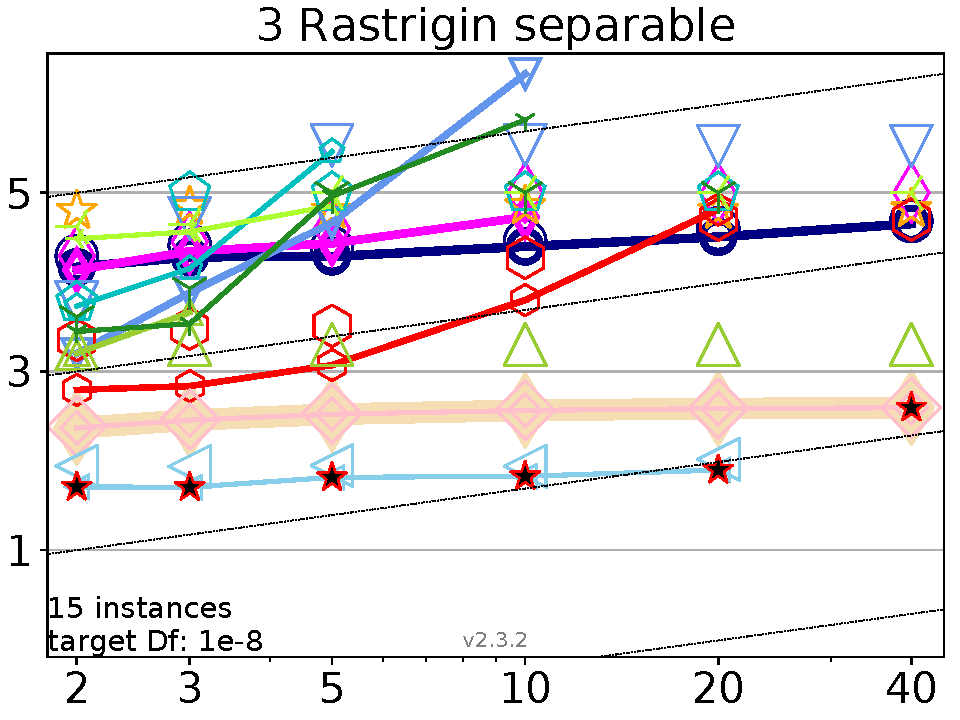
\includegraphics[width=0.28\textwidth]{ppfigs_f003}\\
        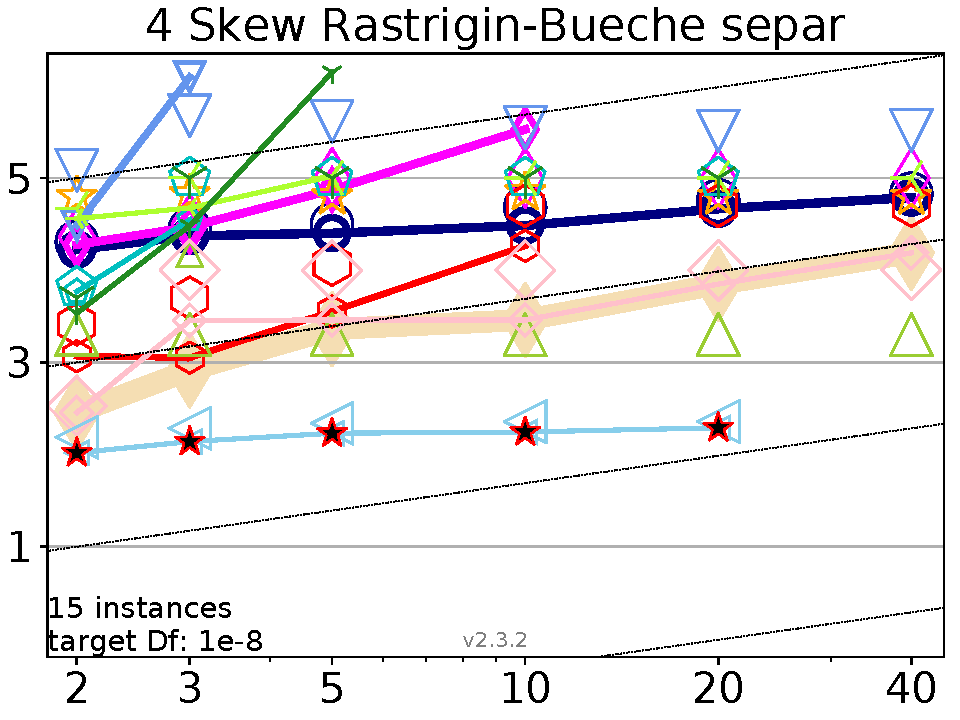
\includegraphics[width=0.28\textwidth]{ppfigs_f004}\\
        
        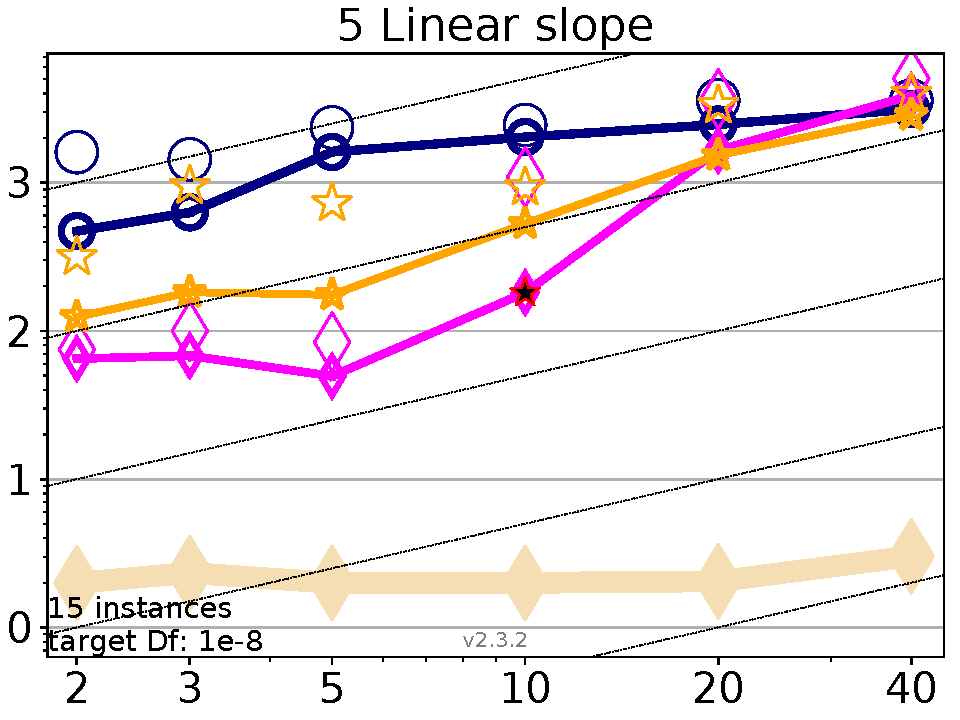
\includegraphics[width=0.28\textwidth]{ppfigs_f005}\\
        \end{tabular}
        \vspace{-3ex}
         \caption{Average running time (in \#FEs as $log_{10}$ value),
          divided by dimension for target function value $10^{-8}$ vs dimension. 
          Algorithms legends are given in $f_1$. Light symbols give the maximum number of 
          function evaluations from the longest trial divided by dimension. 
          Black stars indicate a statistically better result compared to 
          all other algorithms ($p < 0.01$) and Bonferroni 
          correction number of dimensions (six).}
    \end{figure}  


\begin{acks}

  The authors would also like to thank the anonymous referees for
  their valuable comments and helpful suggestions. The work is
  supported by the \grantsponsor{GS501100001809}{XXXXXX XXX
    XXXX} under Grant
  No.:~\grantnum{GS5SAAA00001809}{61273304}
  and~\grantnum[http://www.nnsf.cn/xxxxxxxx]{G1100001809}{XXXX XXXXX}.

\end{acks}
